\begin{frame}{Deep Learning: High-level}

Usual paradigm:
%
\begin{itemize}
\item we want to find a \textbf{model} that gives target \textbf{outputs} for particular \textbf{inputs},
\item we represent the model as a \textbf{function of parameters},
\begin{equation*}
f_{\theta}(x) = W_2 \sigma\left( W_1 x + b_1 \right) + b_2, \;\;\;\;\; \theta = \{W_1, W_2, b_1, b_2\}
\end{equation*}
\item we can evaluate the model performance with a \textbf{differentiable loss function} that depends on \textbf{a set of data},
\begin{equation*}
\calL(\theta) = \frac{1}{|\calD|}\sum_{(x,y)\in\calD} L(x,y,f_{\theta}(x))
\end{equation*}
\item and we find the optimal model by \textbf{gradient descent on the loss}.
\begin{equation*}
\theta \leftarrow \theta - \alpha \nabla_{\theta} \calL(\theta)
\end{equation*}
\end{itemize}

\end{frame}

\begin{frame}{Deep Learning: What makes it deep?}

\begin{itemize}
\item ``Deep" refers to using \textbf{function composition} as the building block for models

\item Deep models have many \textbf{layers}: output of one layer is input to next
\end{itemize}


\twocolumns{0.5}{0.5}{
\begin{figure}
\centering
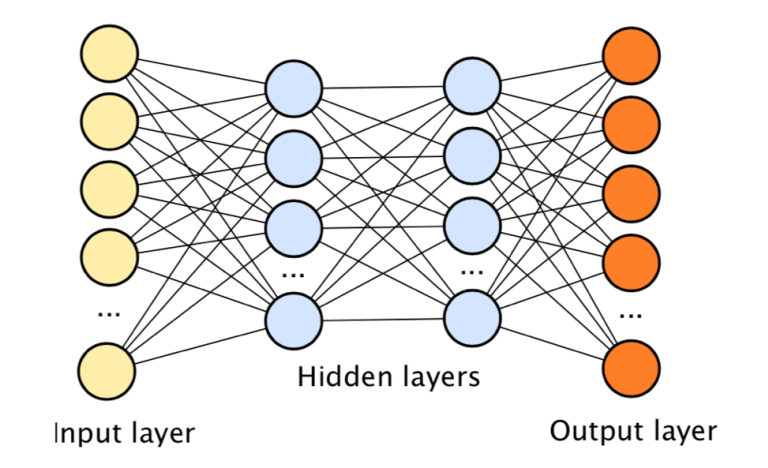
\includegraphics[width=0.8\textwidth]{deep-neural-networks}
\end{figure}
\begin{figure}
\centering
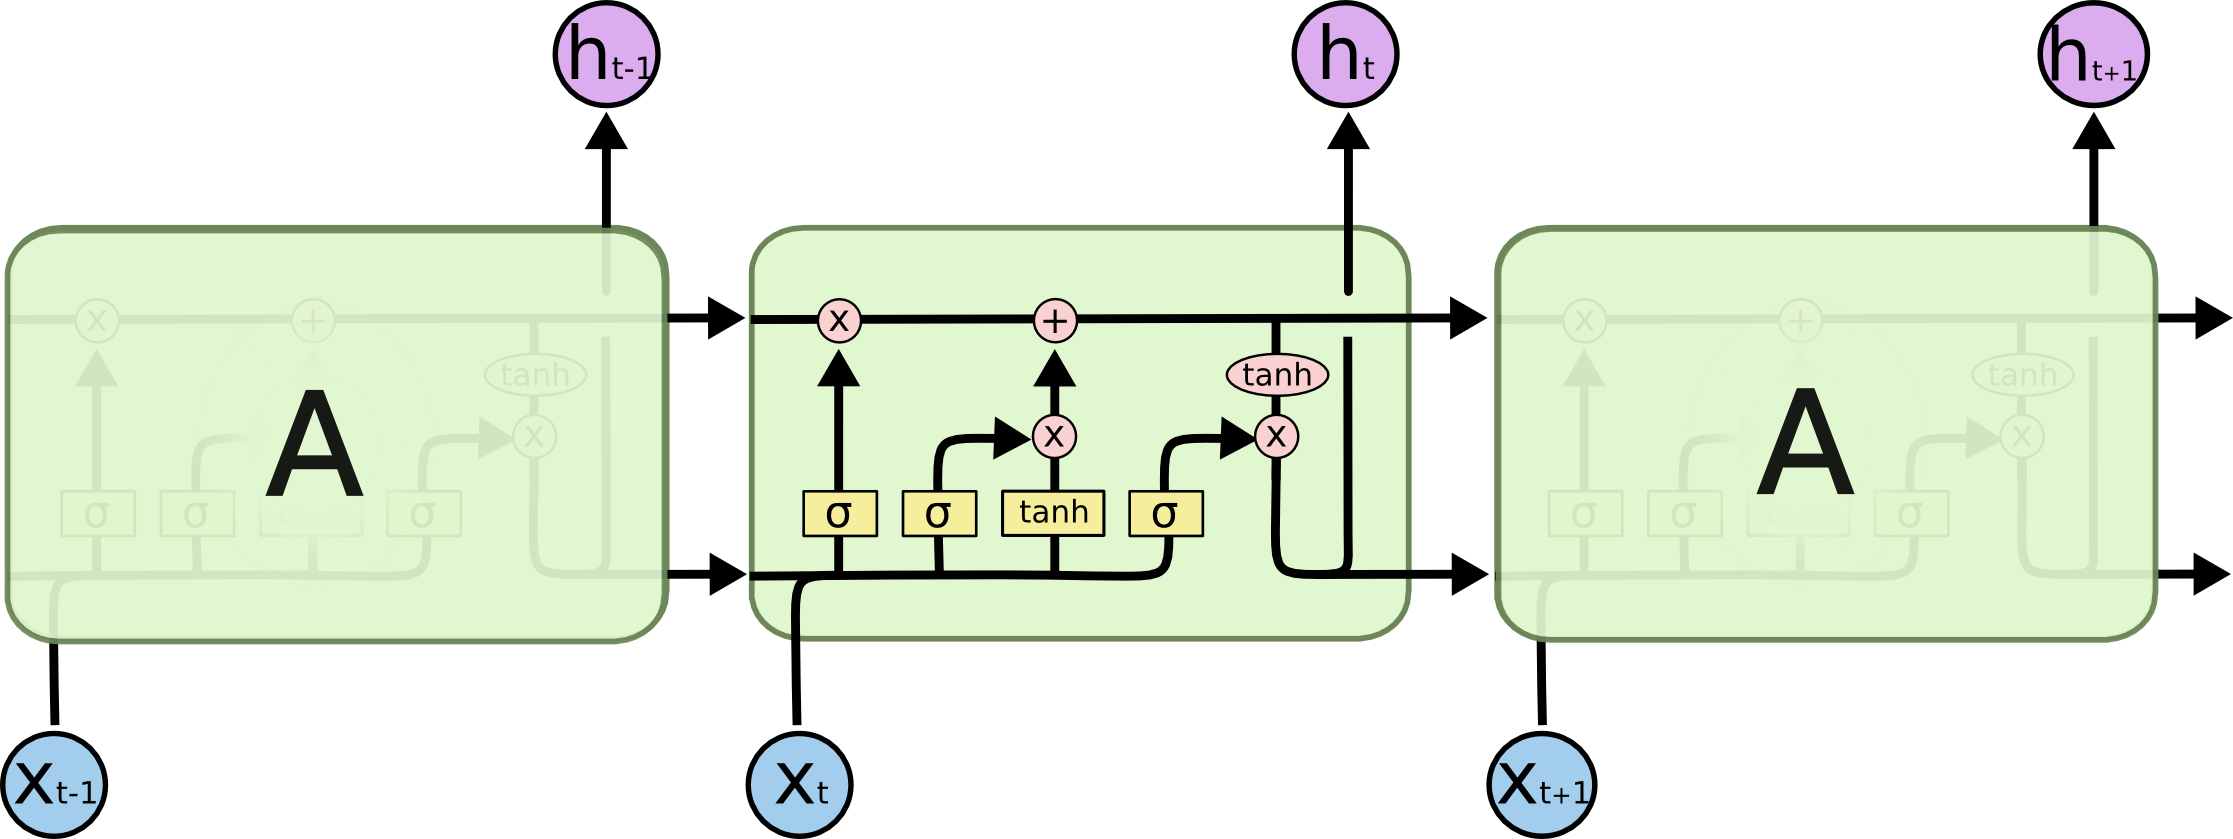
\includegraphics[width=0.8\textwidth]{dl-colah-lstm}
\end{figure}
}{
\begin{figure}
\centering
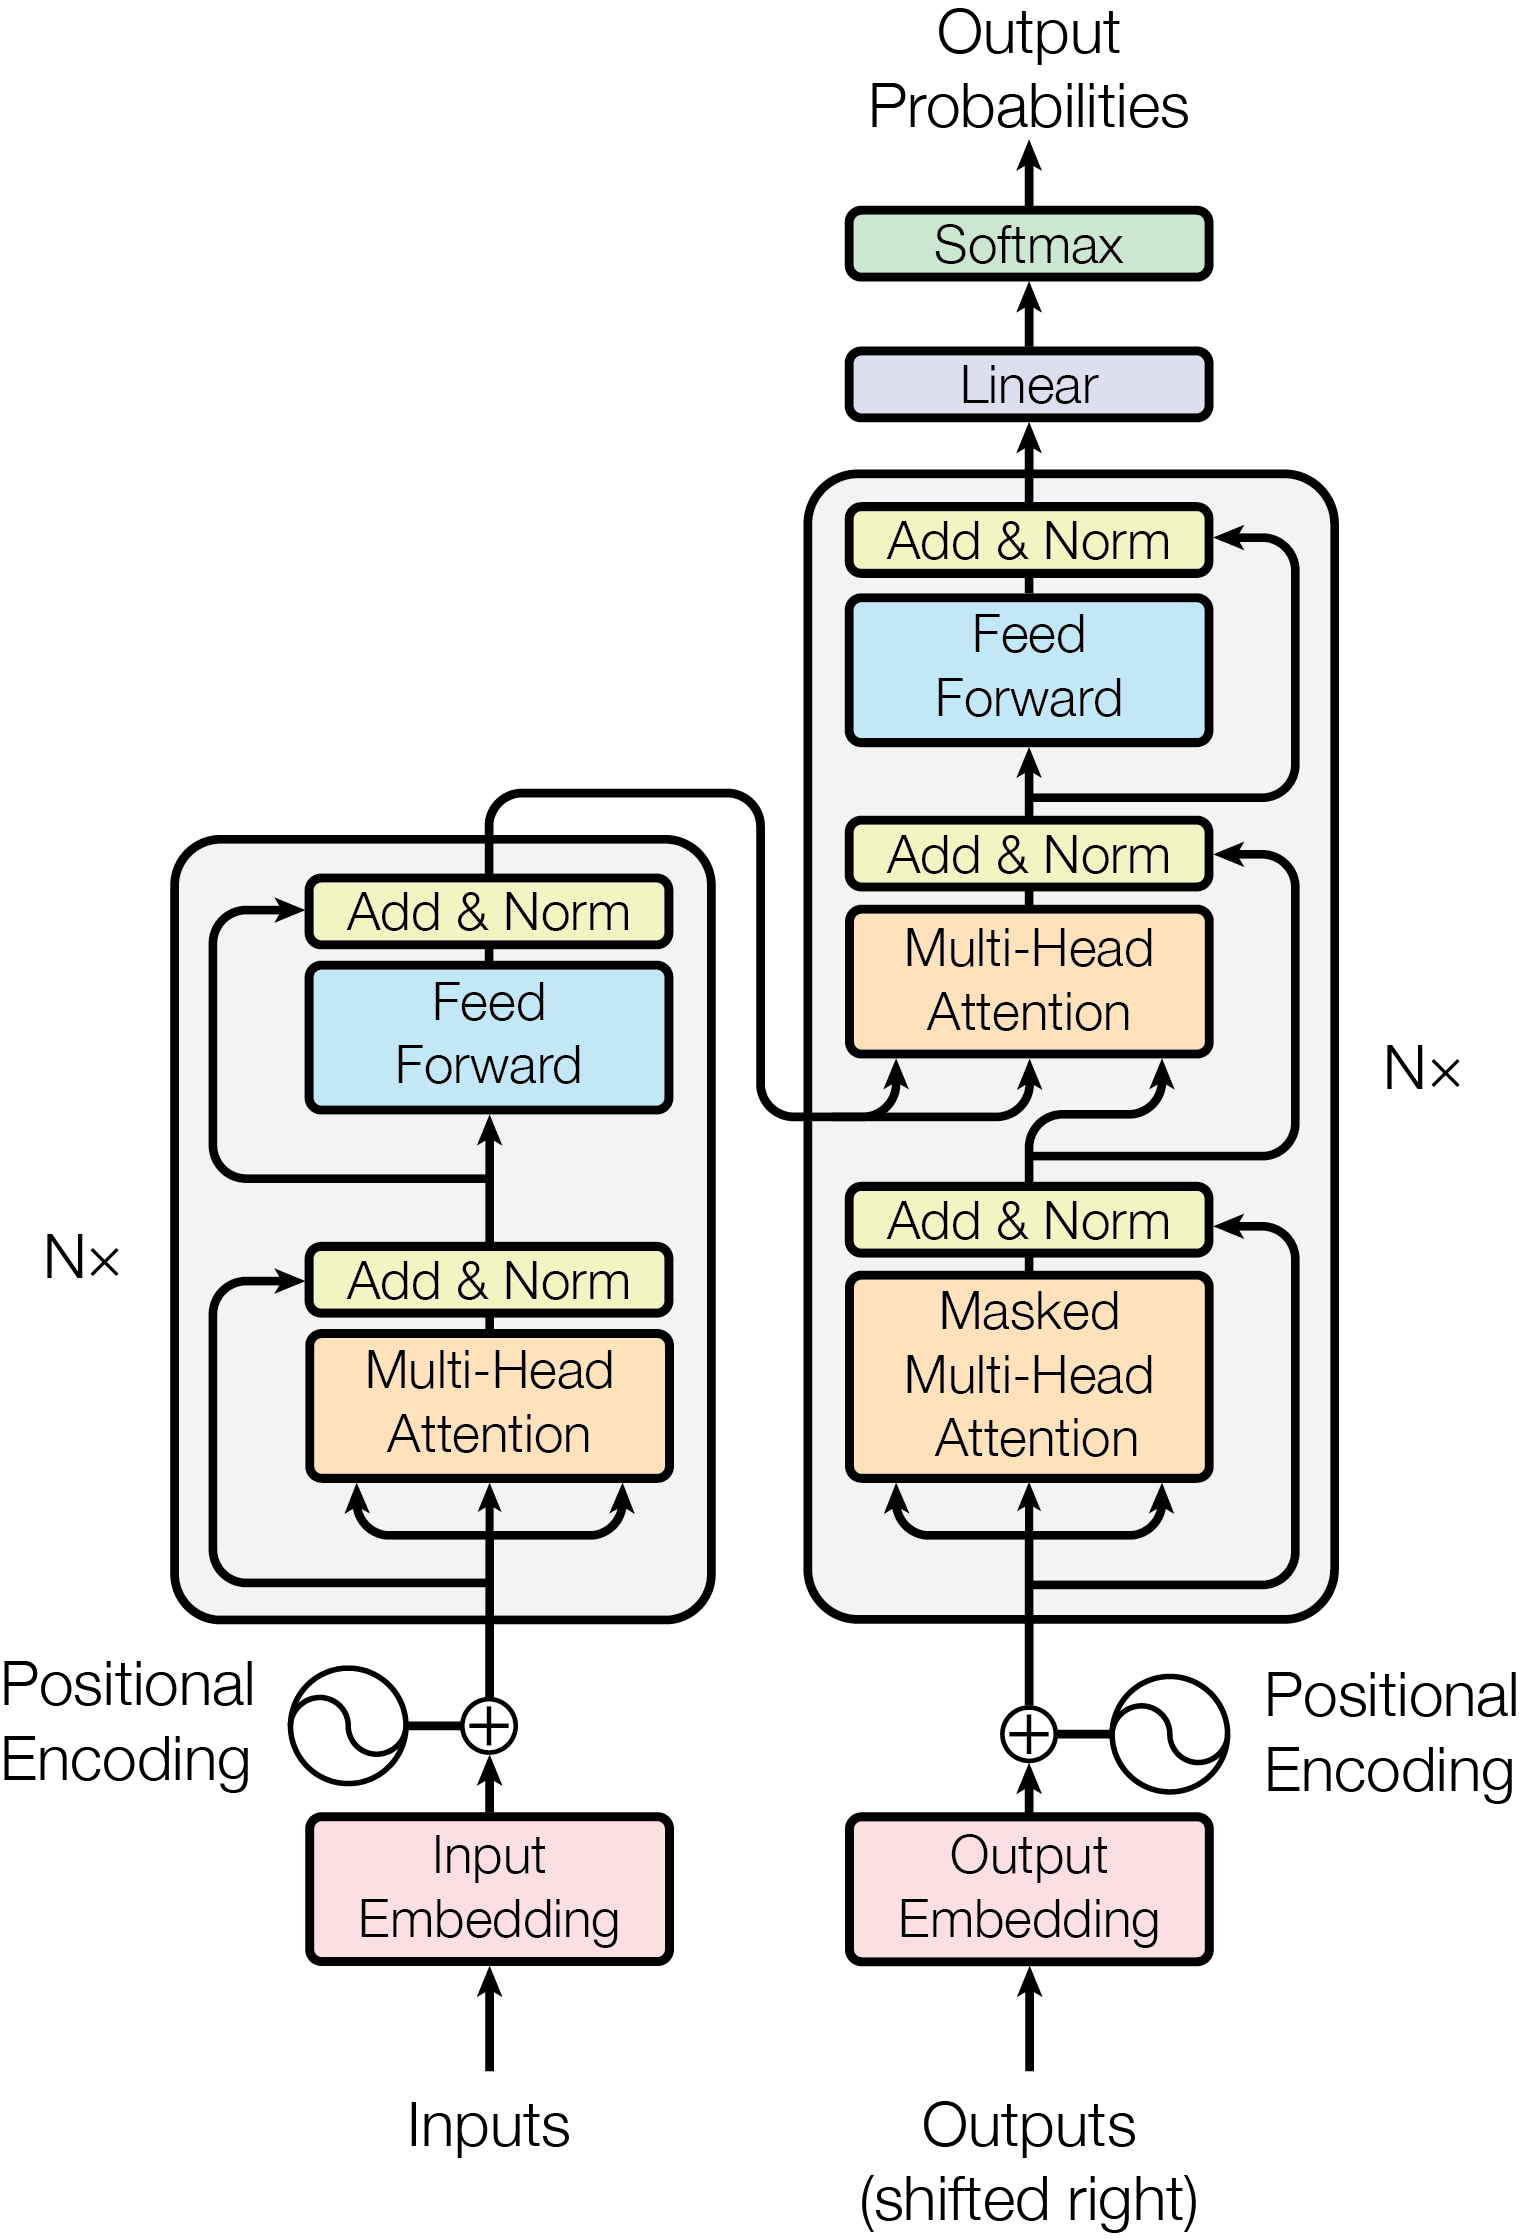
\includegraphics[height=6cm]{dl-transformer}
\end{figure}
}

\footnotetext[1]{MLP credit: Gary Marcus, LSTM credit: Chris Olah, Transformer credit: Vaswani et al 2017}
\end{frame}

\begin{frame}{Deep Learning: What else?}

\begin{itemize}
\item Regularizers make optimization problems better-behaved:
\begin{equation*}
\calL(\theta) \to \calL(\theta) + \lambda \Omega(\theta)
\end{equation*}
\item Normalization makes optimization easier:
\begin{equation*}
a \to \frac{g}{\sigma}\left(a - \mu\right) + b
\end{equation*}
\item Adaptive optimizers (eg Adam) makes optimization faster:
\begin{align*}
m &\leftarrow \beta_1 m + (1-\beta_1) g \\
v &\leftarrow \beta_2 v + (1-\beta_2) g^2 \\
\theta &\leftarrow \theta - \alpha \frac{m}{\sqrt{v}+\epsilon}
\end{align*}
\item Reparameterization trick comes in handy sometimes:
%
\begin{equation*}
\underE{x \sim p_{\theta}}{F(x)} = \underE{z \sim \calN}{F(\xi(\theta, z))}
\end{equation*}
\item For links to detailed resources, see the Spinning Up essay!
\end{itemize}

\end{frame}